\section{The Attractiveness-Optionality Conjecture}
\label{sec:conjecture}

Superposition across multiple concurrent partners is costly to coordinate. Why do some
individuals regularly inhabit distributed portfolios while others collapse rapidly onto
monogamous matches? This section separates the exact discrete probability of multi-option
retention (\layermath{}), including heterogeneous and attention-budget-capped extensions,
from the empirical hypothesis linking option supply to attractiveness (\layerempiric{}).

\subsection{Discrete Retention Models Beyond I.I.D.\ Binomial}
\label{subsec:conj-model}

\noindent\layerformal{} Let $n \in \Nnum$ denote the focal agent's active or accessible
pool of mutually interested, non-exclusive options during a baseline window, and suppose
each viable partner $i \in \{1, \dots, n\}$ remains concurrently retained without collapsing
with probability $p_i \in [0, 1]$. Under the minimal baseline model with homogeneous
independent probabilities $p_i = p$, the retained active count $K = \sum_{i=1}^n X_i$ follows
$\operatorname{Binomial}(n, p)$.

\begin{definition}[Binomial superposition probability; \layermath]
\label{def:binomial-superposition}
For $n \ge 0$ and $p \in [0, 1]$, define the multi-partner superposition probability
\begin{equation}
  P_{\mathrm{sup}}(n, p) = \Prob(K \ge 2)
  = \begin{cases}
    0 & n \in \{0, 1\}, \\[4pt]
    1 - (1 - p)^n - n p (1 - p)^{n-1} & n \ge 2.
  \end{cases}
  \label{eq:binomial-superposition}
\end{equation}
\end{definition}

\begin{theorem}[Monotonicity and exact marginal step; \layermath]
\label{thm:optionality-monotonicity}
For every $p \in [0, 1]$ and $n \ge 1$, the increment in superposition probability from
adding one viable partner satisfies
\begin{equation}
  P_{\mathrm{sup}}(n + 1, p) - P_{\mathrm{sup}}(n, p) = n\, p^2 (1 - p)^{n-1} \;\ge\; 0,
  \label{eq:marginal-gain}
\end{equation}
with strict positivity whenever $p \in (0, 1)$. Consequently, $P_{\mathrm{sup}}(n, p)$ is
monotonically non-decreasing in $n$ (and strictly increasing on $n \ge 1$ for $p \in (0, 1)$).
\end{theorem}
\begin{proof}
Algebras of~\eqref{eq:marginal-gain} reduce identically by shifting $(1-p)^{n+1}$ and $(1-p)^n$;
non-negativity and strict positivity follow because $n \ge 1$ and $p, 1-p \ge 0$. Machine-checked
without approximation as \texttt{superpositionProb\_step}, \texttt{superpositionProb\_mono},
and \texttt{superpositionProb\_strict\_step} in \texttt{RST.Optionality.Binomial}.
\end{proof}

\noindent\layermath{} Letting retention probabilities $p_1, \dots, p_n \in [0, 1]$ vary
independently across partners gives a Poisson-binomial count $K = \sum_{i=1}^n X_i$ with mean $\mu = \sum_{i=1}^n p_i$ and variance
$\operatorname{Var}(K) = \sum_{i=1}^n p_i(1 - p_i) \le n/4$ (checked in
\texttt{Optionality.\allowbreak{}Bernoulli}). When total active attention faces a strict
time-budget constraint ($K_{\mathrm{cap}} = \min(K, B_{\max})$ or negatively correlated
crowding once $k \ge B_{\max}$), mean active count saturates sublinearly in $n$.
\cref{fig:optionality-extensions} compares homogeneous Binomial scaling against heterogeneous
Beta-spread weights and capacity-capped sequential thinning ($B_{\max} = 3$).

\begin{figure}[htbp]
  \centering
  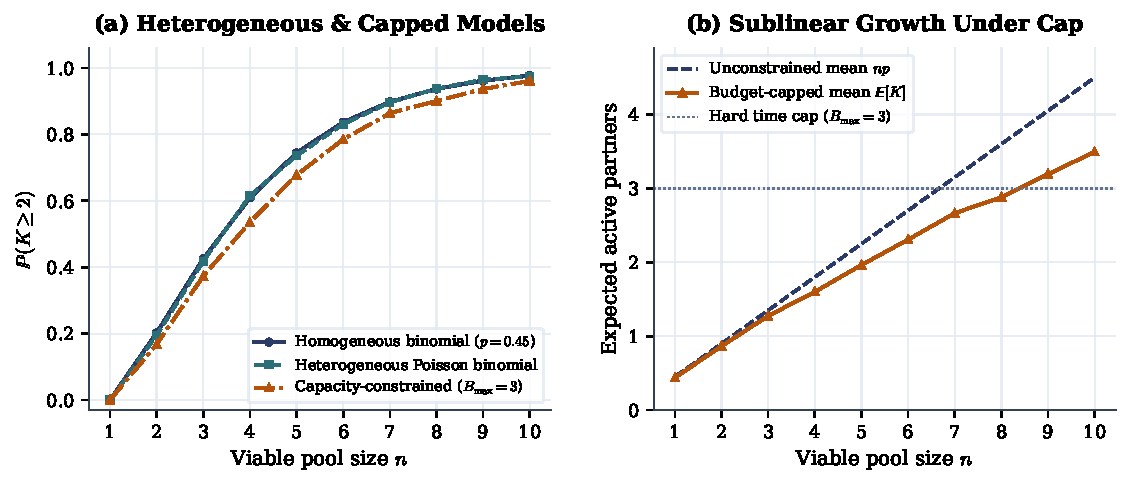
\includegraphics[width=0.92\textwidth]{figures/fig_optionality_extensions.pdf}
  \caption{Extensions of the baseline retention model (Seed \texttt{202602}, $4{,}000$ trials
  per point). (a)~$\Prob(K \ge 2)$ under homogeneous Binomial ($p = 0.45$), heterogeneous
  Poisson-binomial, and attention-budget crowding ($B_{\max} = 3$). (b)~Mean active partners
  versus unconstrained linear scaling $np$.}
  \label{fig:optionality-extensions}
\end{figure}

When candidate pool arrival itself is random with $N \sim \operatorname{Poisson}(\lambda(A))$,
Poisson thinning (\cref{lem:app-poisson}) yields unconditionally
\begin{equation}
  P_{\mathrm{sup}}^{\mathrm{Poi}}(\lambda, p)
  = \Prob(K \ge 2) = 1 - e^{-p\lambda}\bigl(1 + p\lambda\bigr),
  \label{eq:poisson-superposition}
\end{equation}
which strictly increases with expected arrival intensity $p\lambda$.

\subsection{The Attractiveness-Optionality Conjecture}
\label{subsec:conj-statement}

\begin{conjecture}[Attractiveness-Optionality Conjecture; \layerempiric]
\label{conj:optionality}
Let $A \ge 0$ denote a population-perceived attractiveness index and let $n(A)$ denote the
corresponding expected count of viable, non-exclusive options accessible to the focal agent.
Assuming $n(A)$ is monotonically increasing in $A$ over an active social market, while
baseline tolerance $p$ stays bounded away from zero, the equilibrium probability of occupying
a superposed multi-partner portfolio scales monotonically with $A$:
\begin{equation}
  A_1 < A_2 \;\implies\; n(A_1) \le n(A_2) \;\implies\;
  \Prob(\text{superposition} \mid A_1) \;\le\; \Prob(\text{superposition} \mid A_2).
  \label{eq:conjecture}
\end{equation}
\end{conjecture}

\noindent\layermath{} Notice the strict boundary of formal proof: theorem
\texttt{conjecture\_mono\_\allowbreak{}in\_attractiveness} in \texttt{Optionality.\allowbreak{}Binomial}
proves \emph{only} the conditional implication $[(\forall A_1 \le A_2,\; n(A_1) \le n(A_2)) \implies
P_{\mathrm{sup}}(n(A_1), p) \le P_{\mathrm{sup}}(n(A_2), p)]$. Whether human partner
arrival counts $n(A)$ actually satisfy that monotonicity, and how strongly confounders
attenuate it, is purely empirical.

\begin{figure}[htbp]
  \centering
  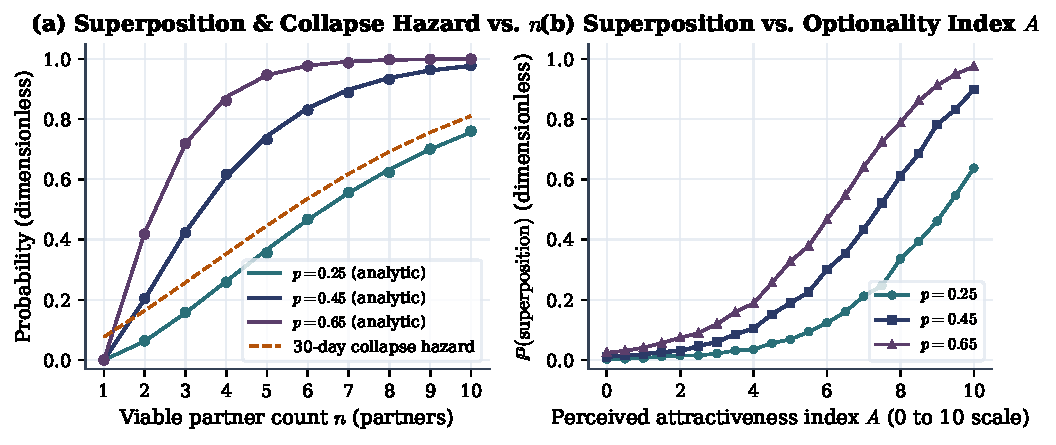
\includegraphics[width=0.92\textwidth]{figures/fig_collapse_vs_n_A.pdf}
  \caption{Synthetic optionality and stability tradeoff (Seed \texttt{202602}).
  (a)~Analytic vs.\ Monte Carlo $\Prob(K \ge 2)$ across $n = 1,\dots,10$ alongside 30-day
  percolation-coupled collapse hazard. (b)~Superposition probability vs.\ perceived
  attractiveness index $A$ under synthetic arrival function $n(A)$.}
  \label{fig:collapse-vs-n-A}
\end{figure}

\subsection{Confounders, Selection Effects, and Empirical Discrimination}
\label{subsec:conj-design}

\noindent\layerempiric{} \layerbehav{} An observed correlation between $A$ and concurrent
partnerships need not confirm \cref{conj:optionality} cleanly unless alternative mechanisms
are separated empirically:
\begin{enumerate}[nosep]
  \item \textbf{Selectivity attenuation.} Higher-$A$ individuals may raise their acceptance
        threshold simultaneously, leaving realized retained count flat despite larger arrival $n(A)$.
  \item \textbf{Relationship-goal heterogeneity.} Sociosexual orientation and commitment
        preferences independently drive both dating strategy and self-selection into multiple chats.
  \item \textbf{Venue and network assortativity.} High-density urban campuses and shared
        social feeds raise both incoming options $n(A)$ and social edge density $q$, amplifying
        decoherence hazard alongside superposition incidence.
\end{enumerate}

\subsection{Utility Versus Systemic Collapse Tradeoff}
\label{subsec:conj-tradeoff}

\noindent\layerbehav{} \layersatire{} As $n$ rises, role-coverage complementarity
(\cref{eq:jensen-portfolio}) saturates with diminishing returns around $n \approx 5$--$7$,
whereas total 30-day social-graph collapse hazard increases convexly from $0.0769$ ($n = 1$)
to $0.8106$ ($n = 10$), producing an interior structural optimum near $n \approx 3$--$5$
concurrent partners before coordination overhead dominates.
